\documentclass{../lab_class}

\usepackage{fancyhdr}
\pagestyle{fancy}
\rhead{П.\,Ю. Смирнов, 687 гр.}
\lhead{Лабораторная работа № 4.7.1, МФТИ, весна 2018}

\begin{document}

{\Large 4.7.1 -- Двойное лучепреломление.}

\paragraph{Цель работы.}
Изучение  зависимости  показателя  преломления необыкновенной волны от направления в двоякопреломляющем кристалле; определение главных показателей преломления в кристалле.

В работе используются: гелий-неоновый лазер, вращающийся столик с неподвижным лимбом, призма из исландского шпата, поляроид.

\paragraph{Теоретическая часть.}
Двойное лучепреломления -- явление, характерное для одноосных кристаллов, типичный пример неизотропной оптики. В неизотропной среде в общем случае векторы $D$ и $E$ неколлинеарны: $D = \varepsilon_{\parallel} E_{\parallel} + \varepsilon_{\perp} E_{\perp}$. Из уравнений Максвелла для гаромнических волн получаем тогда
$$
	\vb{D} = -\frac{c}{\omega} \vb{k} \times \vb{H}, \quad \vb{H} = \frac{c}{\omega} \vb{k} \times \vb{E}.
$$
Видим, что векторы $\vb{D}, \vb{H}, \vb{k}$ взаимно перпендикулярны. Поскольку в анизотропной среде $\vb{D}$ не коллинеарен $\vb{E}$, то получаем, что вектор Пойнтинга $\vb{S} = 4\pi/c \vb{E} \times \vb{H}$ (направление распространения энергии) не коллинеарен волновому вектору (распространение фронта волны)! Рассматривая полученный результат вместе с материальным уравнением, видим, что возможны лишь два случая -- вектор $\vb{D}$ перпенд. плоскости оптической оси кристалла и волнового вектора, либо же он лежит в главном сечении. В первом случае фазовая скорость не зависит от направления волнового вектора и равна $v = \omega / k = c / n_o$; такую волну называют \emph{обыкновенной}, она ничем не отличается от плоской волны в изотропной среде. Во втором случае квадрат коэффициента преломления есть отношение вектора $D$ и проекции $E$ на его направление, потому
$$
	n_e = \frac{1}{\frac{\sin^2 \theta}{\varepsilon_{\parallel}} + \frac{\cos^2 \theta}{\varepsilon_{\perp}}},
$$
где $\theta$ -- угол между осью кристалла и $\vb{E}$. Соотв. фазовая скорость зависит от угла; такую волну называют \emph{необыкновенной}. В общем случае всякая волна раскладывается в суперпозицию указанных типов волн.

В нашем опыте мы измеряем характеристики кристалла, используя призму. 

\paragraph{Эксперимент.}

По полученным данным (см. таблицы в .ipynb) строим графики $n_o$ и $n_e$ от $\cos^2 \theta$ в Sigma Plot.

\begin{figure}[H]
	\centering
	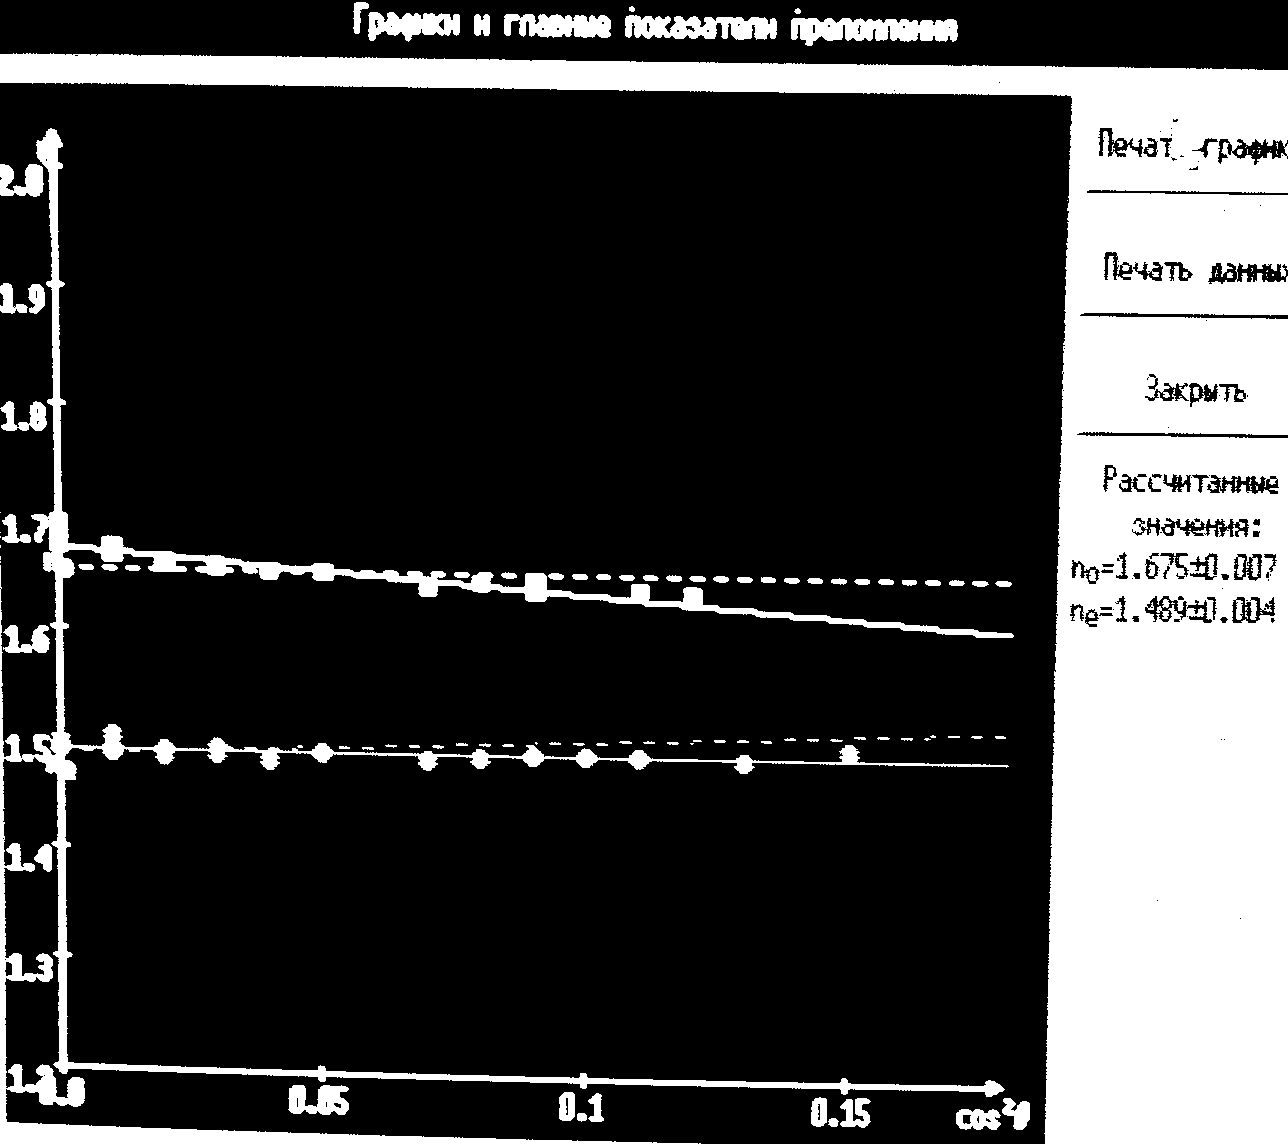
\includegraphics[width = 0.5\textwidth]{screen.png}
	\caption{Графики и главные показатели преломления.}
\end{figure}

Из графиков получаем значения
\begin{gather*}
	n_o = 1.675 \pm 0.017, \\
	n_e = 1.489 \pm 0.013,
\end{gather*}
что хорошо согласуется с табличными данными. 

Рассчитаем средние значения углов наименьшего отклонения
\begin{gather*}
	\psi_{mo} = 26 \pm 1^{\circ}, \\
	\psi_{me} = 21 \pm 1^{\circ}.
\end{gather*}

Расчёты показателей преломления с помощью универсальной зависимости дают
\begin{gather*}
	n_o = 1.67 \pm 0.03, \\
	n_e = 1.5 \pm 0.04.
\end{gather*}

Углы падения, соответствующие полному внутреннему отражению:
\begin{gather*}
	\varphi_{1o} = 2.5 \pm {0.5}^{\circ}, \\
	\varphi_{1e} = 5.0 \pm {0.5}^{\circ}.
\end{gather*}

Через углы наименьшего отклонения определяем
\begin{gather*}
	n_o = 1.65 \pm 0.07, \\
	n_e = 1.48 \pm 0.06.
\end{gather*}

\begin{table}[]
\fontsize{20pt}{30pt}
\centering
\resizebox{\textwidth}{!}{%
\begin{tabular}{lllllllllllllllllllllllllll}
$\varphi_o$ & 3.25  & 4  & 5.75  & 9.25  & 16  & 7.5  & 11.5  & 5  & 7.5  & 10  & 12.5  & 15  & 17.5  & 20  & 22.5  & 25  & 26.25  & 27.5  & 28.75  & 30  & 32.5  & 35  & 40  & 45  & 50  & 55 \\
$\psi_o$ & 50  & 45  & 40  & 35  & 30  & 37  & 33  & 42  & 36.5  & 34.5  & 32  & 30.5  & 29.5  & 28.5  & 28  & 27  & 27  & 27  & 27  & 26.5  & 26.5  & 26.5  & 27  & 30  & 31  & 31.5 \\
$\psi_e$ & 26  & 25.5  & 24.5  & 23  & 21  & 24.5  & 22  & 25  & 23.5  & 22.5  & 22  & 21.5  & 20.5  & 20.5  & 20  & 20  & 20  & 20  & 20  & 20  & 20  & 20.5  & 21  & 24.5  & 25.5  & 26 \\
$\cos \theta_o$ & 0  & 0  & 0  & 0.01  & 0.03  & 0.01  & 0.01  & 0  & 0.01  & 0.01  & 0.02  & 0.02  & 0.03  & 0.04  & 0.05  & 0.07  & 0.07  & 0.08  & 0.09  & 0.09  & 0.11  & 0.12  & 0.15  & 0.17  & 0.20  & 0.24 \\
$\cos \theta_e$ & 0  & 0  & 0  & 0.01  & 0.03  & 0.01  & 0.02  & 0  & 0.01  & 0.01  & 0.02  & 0.03  & 0.04  & 0.05  & 0.07  & 0.08  & 0.09  & 0.10  & 0.10  & 0.11  & 0.13  & 0.15  & 0.18  & 0.20  & 0.24  & 0.28 \\
$n_o$ & 1.691  & 1.685  & 1.678  & 1.670  & 1.656  & 1.673  & 1.667  & 1.683  & 1.667  & 1.672  & 1.661  & 1.657  & 1.657  & 1.652  & 1.653  & 1.640  & 1.643  & 1.646  & 1.648  & 1.638  & 1.639  & 1.638  & 1.640  & 1.694  & 1.693  & 1.670 \\
$n_e$ & 1.491  & 1.490  & 1.49  & 1.490  & 1.486  & 1.503  & 1.485  & 1.492  & 1.487  & 1.486  & 1.490  & 1.492  & 1.481  & 1.489  & 1 483  & 1.487  & 1.488  & 1.489  & 1.489  & 1.489  & 1.487  & 1.496  & 1.497  & 1.563  & 1.561  & 1.539
\end{tabular}%
}
\end{table}

\paragraph{Вывод.}
Изучив явление двойного лучепреломления, мы измерили главные показатели преломления тремя различными способами и получили их взаимное согласие в пределах погрешностей.

\end{document}